%
% Copyright 2018 Joel Feldman, Andrew Rechnitzer and Elyse Yeager.
% This work is licensed under a Creative Commons Attribution-NonCommercial-ShareAlike 4.0 International License.
% https://creativecommons.org/licenses/by-nc-sa/4.0/
%
\graphicspath{{figures/cartesian/}}

\section{Cartesian Coordinates}

Each point in two dimensions may be labeled by two coordinates
$(x,y)$ which specify the position of the point in some units with respect
to some axes as in the figure below.
\begin{efig}
\begin{center}
   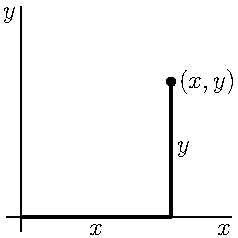
\includegraphics{point2d}
\end{center}
\end{efig}
The set of all points in two dimensions is denoted $\bbbr^2$.
Observe that
\begin{itemize}\itemsep1pt \parskip0pt \parsep0pt
\item the distance from the point $(x,y)$ to the $x$--axis is $|y|$
\item the distance from the point $(x,y)$ to the $y$--axis is $|x|$
\item the distance from the point $(x,y)$ to the origin $(0,0)$ is
     $\sqrt{x^2+y^2}$
\end{itemize}

Similarly, each point in three dimensions may be labeled by
three coordinates $(x,y,z)$, as in the two figures below.
\begin{efig}
\begin{center}
   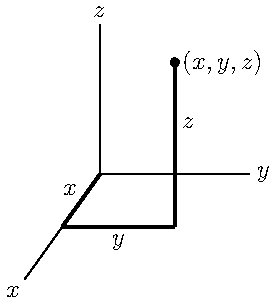
\includegraphics{point3d}\qquad
   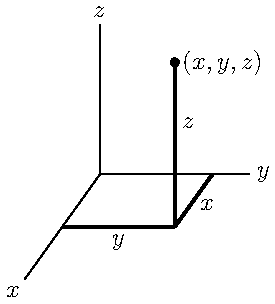
\includegraphics{point3db}
\end{center}
\end{efig}
The set of all points in three dimensions is denoted $\bbbr^3$.
The plane that contains, for example, the $x$-- and $y$--axes
is called the $xy$--plane.
\begin{itemize}\itemsep1pt \parskip0pt \parsep0pt
\item The $xy$--plane is the set of all points $(x,y,z)$ that
obey $z=0$.
\item The $xz$--plane is the set of all points $(x,y,z)$ that
obey $y=0$.
\item The $yz$--plane is the set of all points $(x,y,z)$ that
obey $x=0$.
\end{itemize}
More generally,
\begin{itemize}\itemsep1pt \parskip0pt \parsep0pt
\item The set of all points $(x,y,z)$ that obey $z=c$ is a plane
that is parallel to the $xy$--plane and is a distance $|c|$ from it.
If $c>0$, the plane $z=c$ is above the $xy$--plane.
If $c<0$, the plane $z=c$ is below the $xy$--plane.
We say that the plane $z=c$ is a signed distance $c$ from the
$xy$--plane.

\item The set of all points $(x,y,z)$ that obey $y=b$ is a plane
that is parallel to the $xz$--plane and is a signed distance $b$ from it.

\item The set of all points $(x,y,z)$ that obey $x=a$ is a plane
that is parallel to the $yz$--plane and is a signed distance $a$ from it.
\end{itemize}
\begin{efig}
\begin{center}
   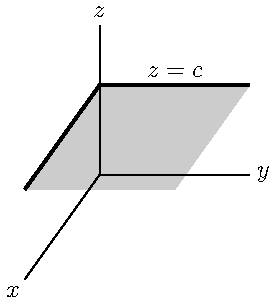
\includegraphics[scale=0.75]{xyplane}\qquad
   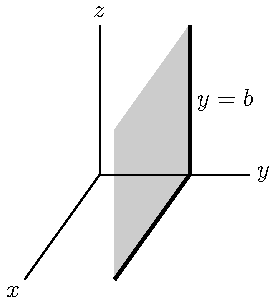
\includegraphics[scale=0.75]{xzplane}\qquad
   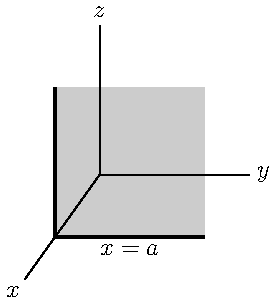
\includegraphics[scale=0.75]{yzplane}
\end{center}
\end{efig}
Observe that
\begin{itemize}\itemsep1pt \parskip0pt \parsep0pt
\item the distance from the point $(x,y,z)$ to the $xy$--plane is $|z|$
\item the distance from the point $(x,y,z)$ to the $xz$--plane is $|y|$
\item the distance from the point $(x,y,z)$ to the $yz$--plane is $|x|$
\item the distance from the point $(x,y,z)$ to the origin $(0,0,0)$ is
     $\sqrt{x^2+y^2+z^2}$
\end{itemize}
The distance from the point $(x,y,z)$ to the point $(x',y',z')$ is
\begin{equation*}
\sqrt{(x-x')^2+(y-y')^2+(z-z')^2}
\end{equation*}
so that the equation of the sphere centered on $(1,2,3)$ with radius $4$,
that is, the set of all points $(x,y,z)$ whose distance from $(1,2,3)$ is $4$,
is
\begin{equation*}
(x-1)^2+(y-2)^2+(z-3)^2=16
\end{equation*}
